\chapter{Diseño}

En este capítulo se va a tratar el diseño del sistema. Encontrando 5 secciones. La primera, Diseño del sistema 6.1, describe la arquitectura general del sistema. La segunda, Diagrama de clases de la aplicación móvil 6.2, describe atributos,los principales métodos y relaciones de la aplicación móvil. La tercera, Diagrama de clases de la aplicación wear 6.3, describe atributos, métodos y relaciones de la aplicación wear. La cuarta sección denominada Casos de uso 6.4, contiene los distintos casos de uso de los usuarios en el sistema. Finalmente, la sección Diseño de la base de datos 6.5, describe la estructura de la base de datos.

\section{Diseño del sistema}

Se pueden diferenciar tres partes principales que interactúan entre ellas. La primera una aplicación Android para el dispositivo wearable que será la encargada de recopilar información y enviarla, la segunda, una aplicación Android móvil la cual recibirá los datos, los procesará y los representará visualmente. La tercera parte formada por un servidor(Firebase), será la encargada de almacenar los datos del usuario y los datos que cree.\\
\\
Así que la estructura del proyecto del cual trata este trabajo,  seguirá el siguiente diseño:

\begin{figure}[H]
	\centering
	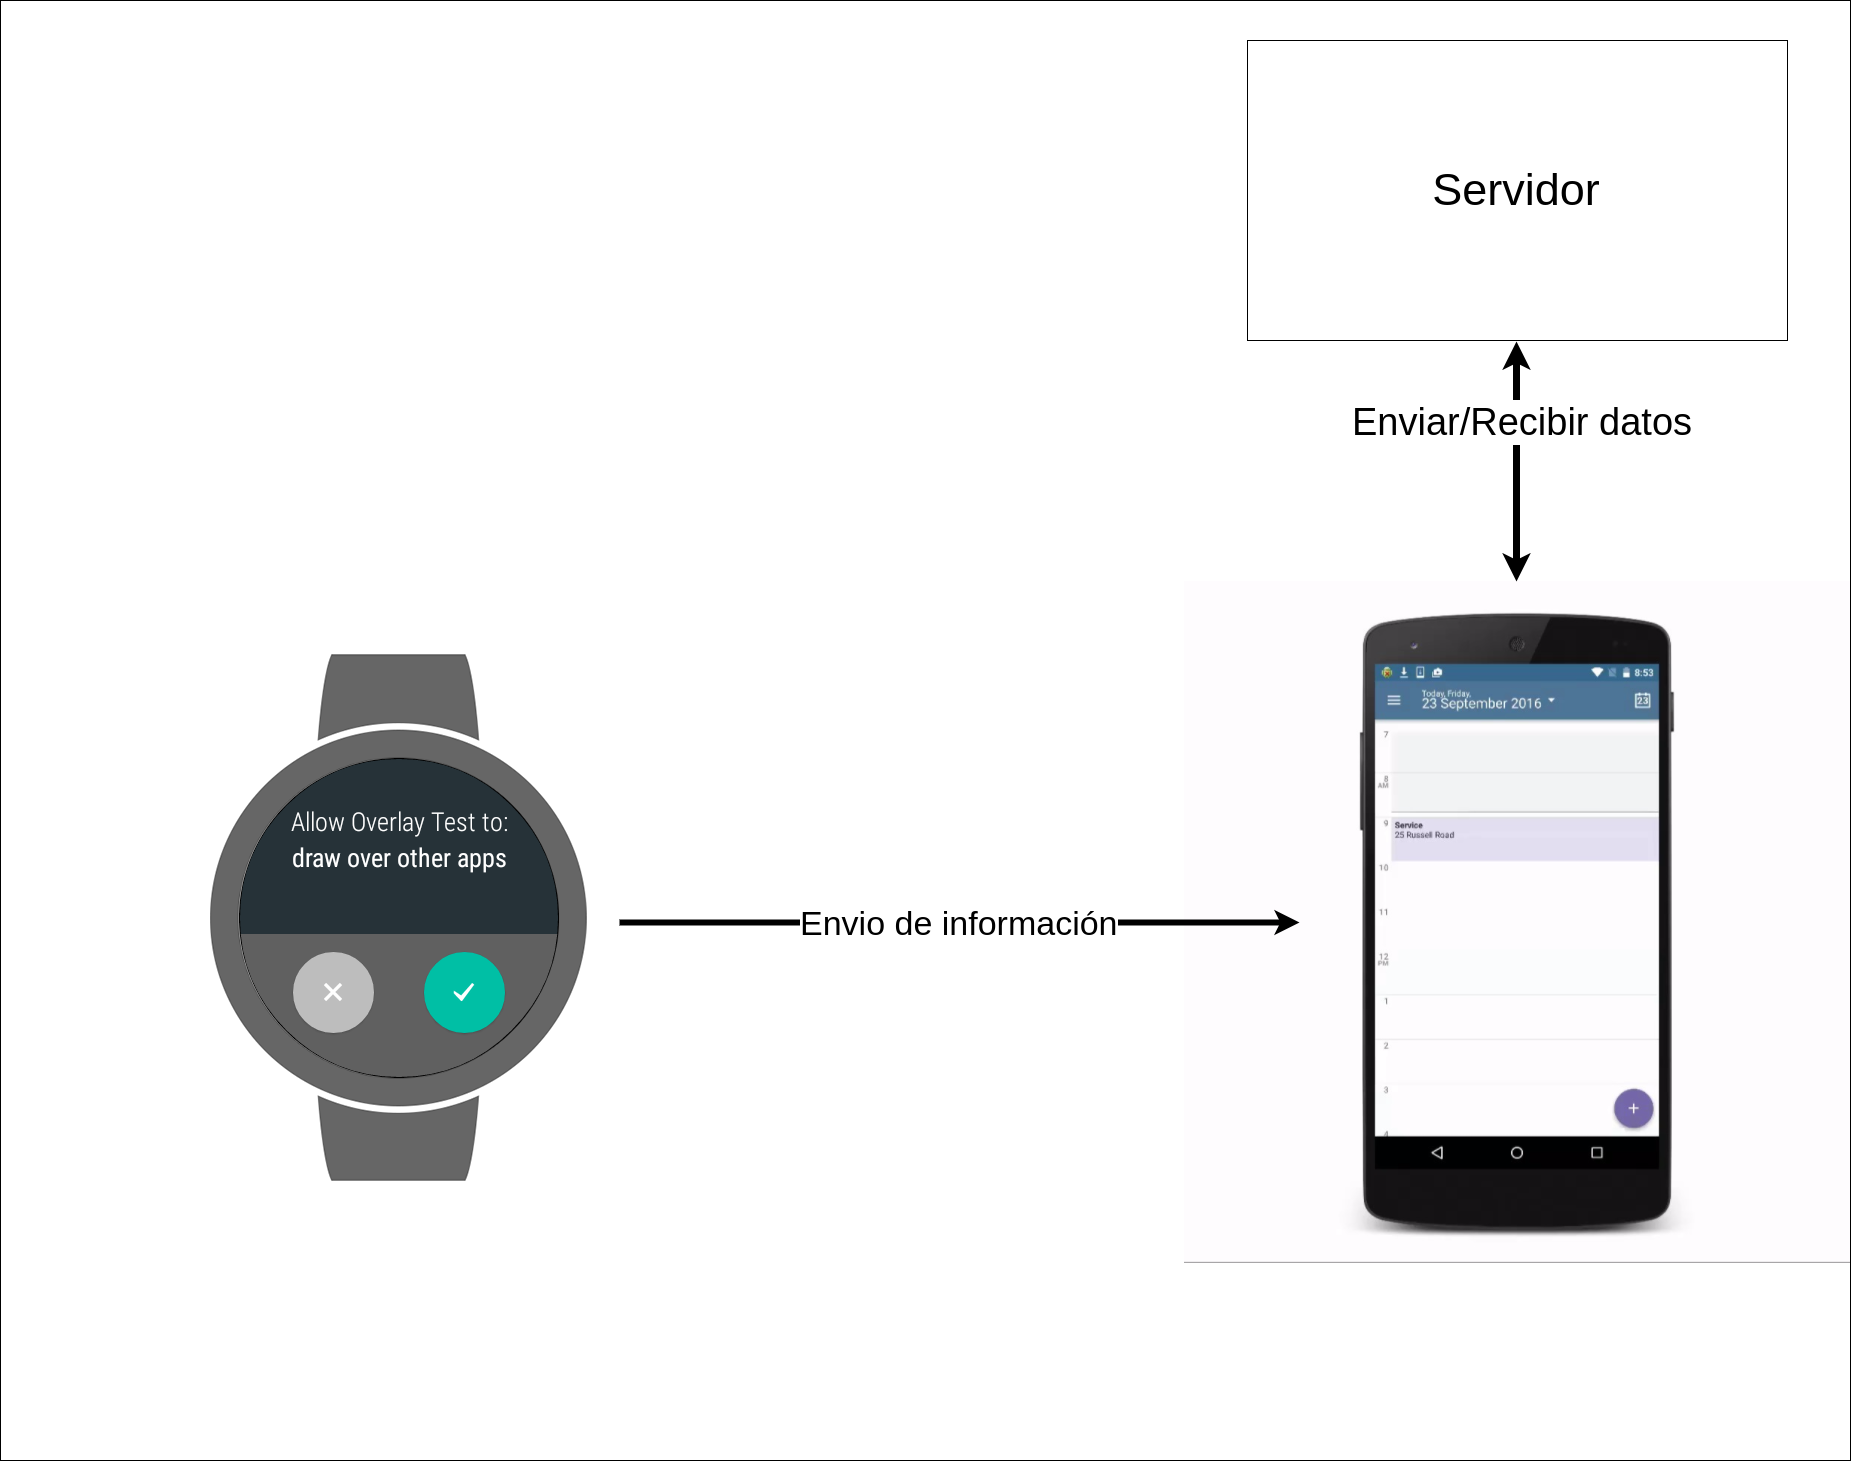
\includegraphics[scale=0.2]{imagenes/disa.png}
	\caption{Arquitectura del proyecto.}
	\label{Arquitectura del proyecto}
\end{figure}
\noindent
En las siguientes secciones de este capítulo se tratará el diseño de cada uno de los componentes de la figura anterior.

\section{Diagrama de clases aplicación móvil}

Esta herramienta describe de manera gráfica utilizando el lenguaje UML las clases y sus relaciones dentro de la aplicación. Otorgando al sistema de todas sus funcionalidades.

\begin{figure}[H]
	\centering
	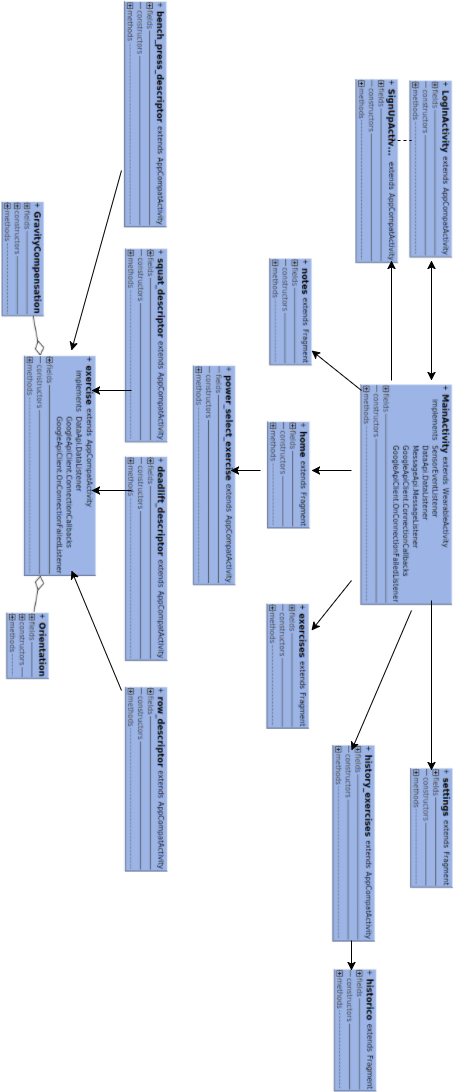
\includegraphics[scale=0.60]{imagenes/clases.jpg}
	\caption{Diagrama de clases de la aplicación móvil.}
	\label{Diagrama de clases android}
\end{figure}

\section{Diagrama de clases aplicación wear}

La finalidad de la aplicación wear es la de recoger y enviar la información, por lo que se ha decidido implementar toda su funcionalidad en una sola clase:

\begin{figure}[H]
	\centering
	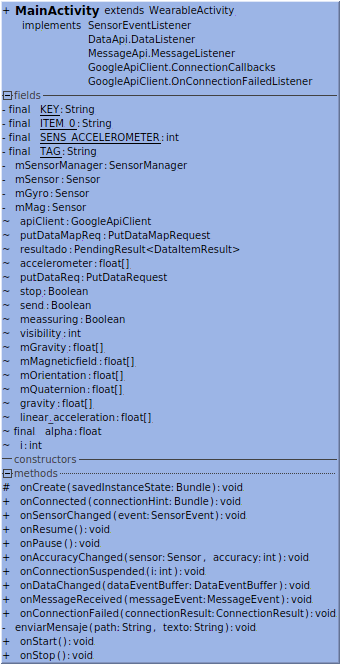
\includegraphics[scale=0.7]{imagenes/clasesW.png}
	\caption{Diagrama de clases de la aplicación wear.}
	\label{Diagrama de clases wear}
\end{figure}

\section{Casos de uso}

En esta sección se va a detallar los casos de uso de la aplicación, los cuales encajan con los requisitos funcionales descritos en el capítulo 3 de este trabajo.\\
\\

\begin{figure}[H]
	\centering
	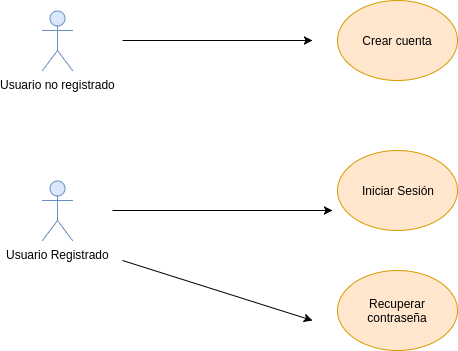
\includegraphics[scale=0.5]{imagenes/uso1.png}
	\caption{Caso de uso 1 - Credenciales.}
	\label{Caso de uso 1}
\end{figure}

\textbf{Crear cuenta}

\begin{table}[h!]
\centering
\caption{Caso de uso - Crear cuenta}
\label{caso de uso crear-cuenta}
\begin{tabular}{|l|l|}
\hline
Titulo         & Crear cuenta                                                                                                                                                                    \\ \hline
Descipción     & \begin{tabular}[c]{@{}l@{}}El usuario puede crearse una cuenta en la aplicación introduciendo \\ el email y una contraseña.\end{tabular}                                        \\ \hline
Actor          & Usuario no registrado                                                                                                                                                           \\ \hline
Precondición   & Que el email no se encuentre ya en el sistema                                                                                                                                   \\ \hline
Secuencia      & \begin{tabular}[c]{@{}l@{}}- El usuario instala la aplicación.\\  - El usuario entra en la aplicación.\\  - Introducir los campos\\  - Pulsar el botón de registro\end{tabular} \\ \hline
Post condición & El usuario entra en la aplicación y ya dispone de credenciales                                                                                                                  \\ \hline
Comentarios    & \begin{tabular}[c]{@{}l@{}}El campo email debe ser un email válido y accesible, pues se \\ utilizará para restaurar la contraseña.\end{tabular}                                 \\ \hline
\end{tabular}
\end{table}

\textbf{Iniciar sesión}
\begin{table}[H]
\centering
\caption{Caso de uso - Inicio sesión}
\label{caso de uso inicio-sesion}
\begin{tabular}{|l|l|}
\hline
Titulo         & Iniciar sesión                                                                                                                                  \\ \hline
Descipción     & \begin{tabular}[c]{@{}l@{}}El usuario podrá iniciar sesión utilizando los credenciales que \\  creó previamente.\end{tabular}                 \\ \hline
Actor          & Usuario registrado                                                                                                                           \\ \hline
Precondición   & Que el usuario se encuentre registrado en el sistema                                                                                            \\ \hline
Secuencia      & \begin{tabular}[c]{@{}l@{}}- El usuario entra en la aplicación\\  - Introducir los campos\\  - Pulsar el botón de inicio de sesión\end{tabular} \\ \hline
Post condición & El usuario se encuentra dentro de la aplicación                                                                                                 \\ \hline
Comentarios    & El usuario debe memorizar su email y contraseña.                                                                                                \\ \hline
\end{tabular}
\end{table}

\textbf{Recuperar contraseña}
\begin{table}[H]
\centering
\caption{Caso de uso - Recuperar contraseña}
\label{caso de uso recuperar-contraseña}
\begin{tabular}{|l|l|}
\hline
Titulo         & Recuperar Contraseña                                                                                                                                 \\ \hline
Descipción     & \begin{tabular}[c]{@{}l@{}}El usuario podrá recupera la contraseña utilizando los credenciales que \\  creó previamente (email).\end{tabular}                 \\ \hline
Actor          & Usuario registrado                                                                                                                           \\ \hline
Precondición   & Que el usuario se encuentre registrado en el sistema                                                                                            \\ \hline
Secuencia      & \begin{tabular}[c]{@{}l@{}}- El usuario entra en la aplicación\\  - Introduce el campo email\\  - Pulsar el botón de recuperar contraseña \\ Accede a su email y recupera la contraseña\end{tabular} \\ \hline
Post condición & El usuario obtiene su contraseña                                                                                                 \\ \hline
Comentarios    & El usuario debe memorizar su email y contraseña.                                                                                                \\ \hline
\end{tabular}
\end{table}

\begin{figure}[H]
	\centering
	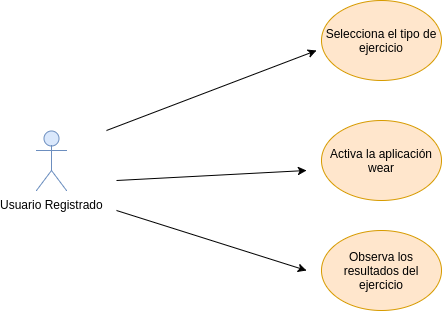
\includegraphics[scale=0.5]{imagenes/uso2.png}
	\caption{Caso de uso 2 - Realización del ejercicio.}
	\label{Caso de uso 2}
\end{figure}

\textbf{Selección del tipo de ejercicio}

\begin{table}[H]
\centering
\caption{Caso de uso - Seleccionar ejercicio}
\label{Caso de uso - Seleccionar ejercicio}
\begin{tabular}{|l|l|}
\hline
Titulo         & Selección del tipo de ejercicio                                                                                                                            \\ \hline
Descipción     & \begin{tabular}[c]{@{}l@{}}El usuario podrá seleccionar el tipo de ejercicio\\ que va a realizar.\end{tabular}                                             \\ \hline
Actor          & Usuario registrado                                                                                                                                         \\ \hline
Precondición   & Que el usuario se encuentre registrado en el sistema                                                                                                       \\ \hline
Secuencia      & \begin{tabular}[c]{@{}l@{}}- El usuario entra en la aplicación\\ - Pulsar la pestaña de ejercicio\\ - Selecciona el tipo de ejercicio deseado\end{tabular} \\ \hline
Post condición & El usuario se encuentra con la descripción del ejercicio                                                                                                   \\ \hline
Comentarios    & \begin{tabular}[c]{@{}l@{}}El usuario debe leer la descripción para realizar el\\ ejercicio correctamente y de manera segura\end{tabular}                  \\ \hline
\end{tabular}
\end{table}

\textbf{Inicio de la monitorización del ejercicio}
\begin{table}[H]
\centering
\caption{Caso de uso - Inicio de la monitorización del ejercicio}
\label{Caso de uso - Inicio de la monitorización del ejercicio}
\begin{tabular}{|l|l|}
\hline
Titulo         & Activar la monitorización de la aplicación wear                                                                                                                                                                              \\ \hline
Descipción     & \begin{tabular}[c]{@{}l@{}}El usuario podrá indicar cuando va a comenzar el \\ ejercicio.\end{tabular}                                                                                                                       \\ \hline
Actor          & Usuario registrado                                                                                                                                                                                                           \\ \hline
Precondición   & \begin{tabular}[c]{@{}l@{}}Que el usuario se encuentre registrado en el sistema y \\ haya seleccionado un ejercicio.\end{tabular}                                                                                            \\ \hline
Secuencia      & \begin{tabular}[c]{@{}l@{}}- El usuario entra en la aplicación\\ - Pulsar la pestaña de ejercicio\\ - Selecciona el tipo de ejercicio deseado\\ - Inicia la aplicación wear.\\ - Selecciona el botón de inicio.\end{tabular} \\ \hline
Post condición & El usuario se encuentra realizando el ejercicio                                                                                                                                                                              \\ \hline
Comentarios    & \begin{tabular}[c]{@{}l@{}}El usuario debe leer la descripción para realizar el\\ ejercicio correctamente y de manera segura\end{tabular}                                                                                    \\ \hline
\end{tabular}
\end{table}

\textbf{Visualización de los resultados}
\begin{table}[H]
\centering
\caption{Caso de uso - Visualización de los resultados }
\label{Visualización de los resultados }
\begin{tabular}{|l|l|}
\hline
Titulo         & Visualización de los resultados                                                                                                                                                                                                                                                           \\ \hline
Descipción     & \begin{tabular}[c]{@{}l@{}}El usuario podrá visualizar la potencia realizada\\ en tiempo real.\end{tabular}                                                                                                                                                                               \\ \hline
Actor          & Usuario registrado                                                                                                                                                                                                                                                                        \\ \hline
Precondición   & \begin{tabular}[c]{@{}l@{}}Que el usuario se encuentre registrado en el sistema, \\ haya seleccionado un ejercicio y haya activado la\\ aplicación wear.\end{tabular}                                                                                                                     \\ \hline
Secuencia      & \begin{tabular}[c]{@{}l@{}}- El usuario entra en la aplicación\\ - Pulsar la pestaña de ejercicio\\ - Selecciona el tipo de ejercicio deseado\\ - Inicia la aplicación wear.\\ - Selecciona el botón de inicio.\\ - Observa como se procesa la información en tiempo\\ real.\end{tabular} \\ \hline
Post condición & El usuario termina la serie.                                                                                                                                                                                                                                                              \\ \hline
Comentarios    & \begin{tabular}[c]{@{}l@{}}El usuario debe leer la descripción para realizar el\\ ejercicio correctamente y de manera segura\end{tabular}                                                                                                                                                 \\ \hline
\end{tabular}
\end{table}


\begin{figure}[H]
	\centering
	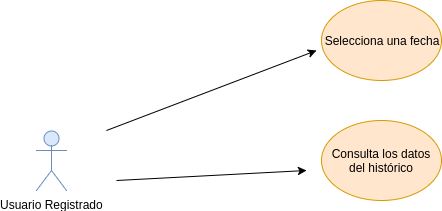
\includegraphics[scale=0.5]{imagenes/uso3.png}
	\caption{Caso de uso 3 - Consulta del histórico.}
	\label{Caso de uso 3}
\end{figure}

\textbf{Selección de una fecha}
\begin{table}[H]
\centering
\caption{Caso de uso - Selección de una fecha}
\label{Caso de uso -  Selección de una fecha}
\begin{tabular}{|l|l|}
\hline
Titulo         & Selección de una fecha                                                                                                                                 \\ \hline
Descipción     & \begin{tabular}[c]{@{}l@{}}El usuario podrá seleccionar una fecha para realizar \\ una consulta.\end{tabular}                                          \\ \hline
Actor          & Usuario registrado                                                                                                                                     \\ \hline
Precondición   & Que el usuario se encuentre registrado en el sistema.                                                                                                  \\ \hline
Secuencia      & \begin{tabular}[c]{@{}l@{}}- El usuario entra en la aplicación\\ - Pulsar la pestaña de historico\\ - Selecciona una fecha del calendario\end{tabular} \\ \hline
Post condición & El usuario visualiza los datos para dicha entrada.                                                                                                     \\ \hline
Comentarios    & \begin{tabular}[c]{@{}l@{}}Si el usuario no realizó ninguna actividad durante \\ dicho día no verá información.\end{tabular}                           \\ \hline
\end{tabular}
\end{table}

\textbf{Consulta de los datos del histórico }
\begin{table}[H]
\centering
\caption{Caso de uso - Consulta de los datos del histórico }
\label{Caso de uso - Consulta de los datos del histórico}
\begin{tabular}{|l|l|}
\hline
Titulo         & Consulta de los datos del histórico                                                                                                                                                               \\ \hline
Descipción     & \begin{tabular}[c]{@{}l@{}}El usuario podrá visualizar su entrenamiento de\\ un día dado.\end{tabular}                                                                                            \\ \hline
Actor          & Usuario registrado                                                                                                                                                                                \\ \hline
Precondición   & \begin{tabular}[c]{@{}l@{}}Que el usuario se encuentre registrado en el sistema y \\ haya seleccionado una fecha.\end{tabular}                                                                    \\ \hline
Secuencia      & \begin{tabular}[c]{@{}l@{}}- El usuario entra en la aplicación\\ - Pulsar la pestaña de historico\\ - Selecciona una fecha del calendario\\ -Visualiza sus datos el dia seleccionado\end{tabular} \\ \hline
Post condición & El usuario visualiza los datos para dicha entrada.                                                                                                                                                \\ \hline
Comentarios    & \begin{tabular}[c]{@{}l@{}}Si el usuario no realizó ninguna actividad durante \\ dicho día no verá información.\end{tabular}                                                                      \\ \hline
\end{tabular}
\end{table}

\section{Diseño de la base de datos}

Como se ha comentado en el capítulo 2 de este documento. La base de datos se va a almacenar en Firebase, que utiliza una estructura no-SQL, utilizando un formato JSON, por lo que se ha decidido almacenar la base de datos de la siguiente manera, con el fin de agilizar la escritura/lectura de los datos de una manera rápida:

\begin{table}[H]
\centering
\caption{Estructura de la base de datos}
\label{Estructura de la base de datos}
\begin{tabular}{|llllll|}
\hline
Usuarios : \{ &           &             &                &      &       \\
         & IdUsuario : \{ &             &                &      &       \\
         &           & FechaActual : \{ &                &      &       \\
         &           &             & Tipo ejercicio : \{ &      &       \\
         &           &             &                & Hora : \{ &       \\
         &           &             &                &      & Datos: [] \\
         &           &             &                &      \}&  \\
         &           &             &               \}&      &  \\
         &           &             \}&               &      &  \\
         &           \}&             &               &      &  \\
         \}&           &             &               &      &  \\
\hline
\end{tabular}
\end{table}
